\item \points{2a}
\textbf{Graphical Analysis.}
\begin{center}
  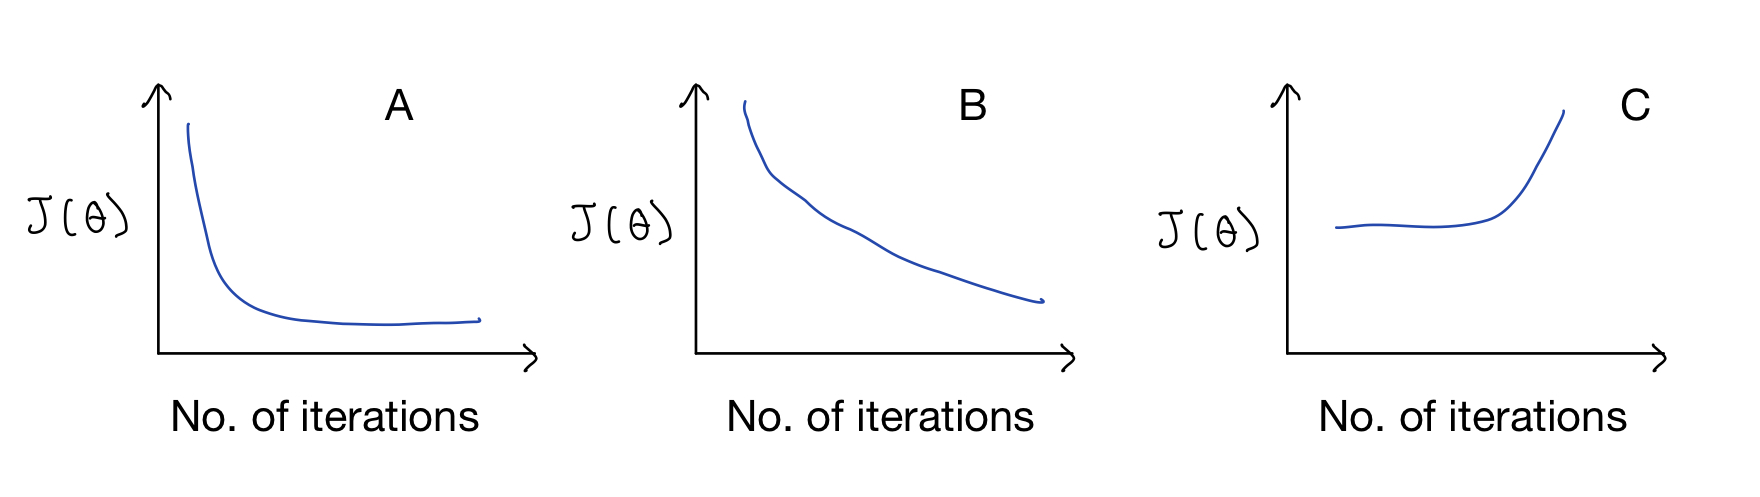
\includegraphics[scale=0.25]{general-ml-theory-tex/IMG_0632.jpg}  
\end{center}
Suppose the above graphs correspond to training the same model on the same data with stochastic gradient descent. Let $l_1$, $l_2$, and $l_3$ be the three learning rates for $A$, $B$, and $C$ respectively. Which of the following is true about $l_1$, $l_2$, and $l_3$? Select one option below.

\begin{enumerate}[label=(\alph*)]
    \item $l_2 < l_1 < l_3$
    \item $l_1 > l_2 > l_3$
    \item $l_1$ = $l_2$ = $l_3$
    \item None of these
\end{enumerate} 
